\chapname = {MAAS in VENV - III : Nodes}

\chapter{\the\chapname}

\section{Creating a few nodes}

There is a restriction on creating virtual machine that it won't let you proceed until you specify an iso file. Hence, create a dummy iso file by using the command: 

\$ touch nothing.iso

We will start creating a single node and then we will clone that to make a few more nodes.

Configurations for creating a new virtual machine with dummy nothing.iso image:

\begin{itemize}
    \setlength\itemsep{0em}
    \item Memory - 1024 MB
    \item CPU Cores - 2
    \item Storage - 20 GB qcow2 
    \item Name - node0
    \item Boot order - 1.) PXE  2.) HDD
    \item Network - maasisotest
    \item NIC Interface 
    \begin{itemize}
        \item Network source - maasisotest
        \item Device model - virtio
    \end{itemize}
    \item Disk bus - virtio
    \item Remove unnecessary virtual hardware from the list for eg. sound
\end{itemize}

\begin{figure}[!ht]
    \centering
    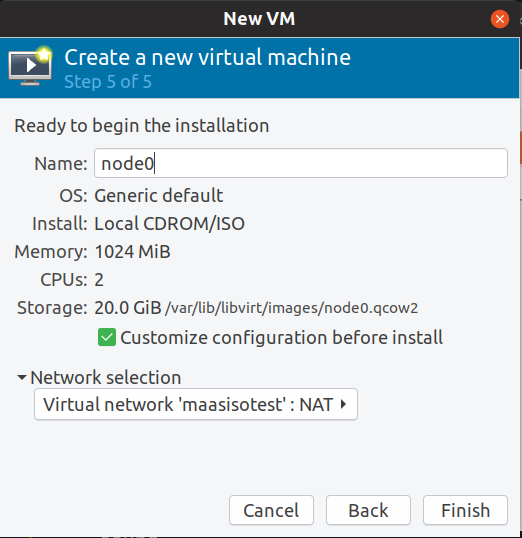
\includegraphics[width=0.5\textwidth]{images/5-1.png}
    \caption{Node 0}
\end{figure}


\begin{figure}[!ht]
    \centering
    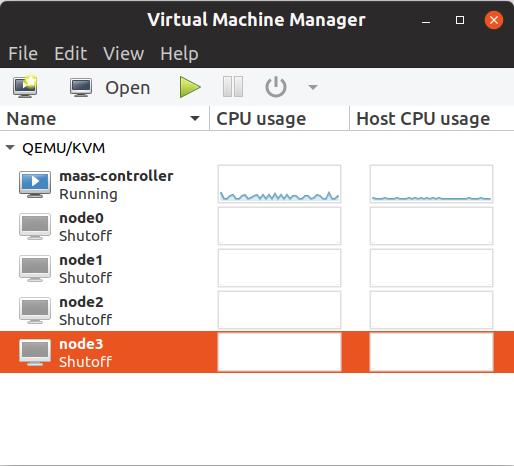
\includegraphics[width=0.5\textwidth]{images/5-2.png}
    \caption{Clones of node 0}
\end{figure}


Begin the installation and once the machine is open, pull the virtual power plug by force off, to create a few virtual machine clones.

Once the clones are created, power on all the virtual machines. These machines will boot for enlistment procedure. They will register themselves and shut themselves down.

\begin{figure}[!ht]
    \centering
    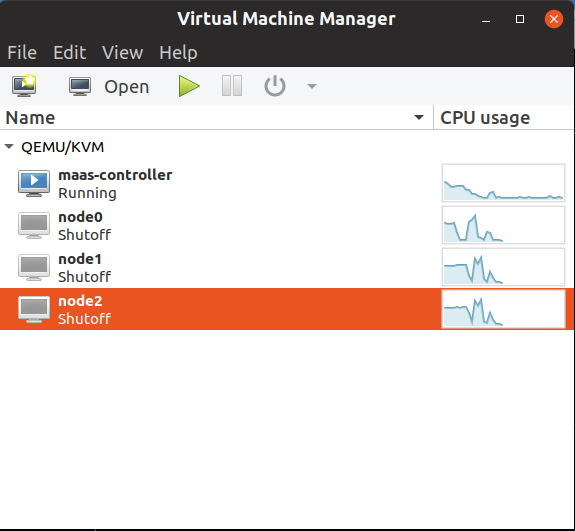
\includegraphics[width=0.7\textwidth]{images/5-3.png}
    \caption{Node enlisting themselves}
\end{figure}

\section{Power configurations}

As soon as they shutdown, we will start configuring the power parameters. Before we do that, we need to change the identifications names of the nodes in the maas interface. 
By default, the node's hostname according to MAAS is a randomly chosen string(Fig. 5.4).

First we need to find the mac address of the interface of a particular node. We can find this in the xml configuration file for the corresponding VM(Fig. 5.5).

\$ virsh dumpxml node0 \textbar grep mac

And then check for the device which has the same mac address in the maas interface and then set the name to node0. In the same way do for the other nodes.

Even though a script can be written to automate this task for the virtual environment case but while operating with the actual hardware there is no other way to completely automate this task.

\begin{figure}[!ht]
    \centering
    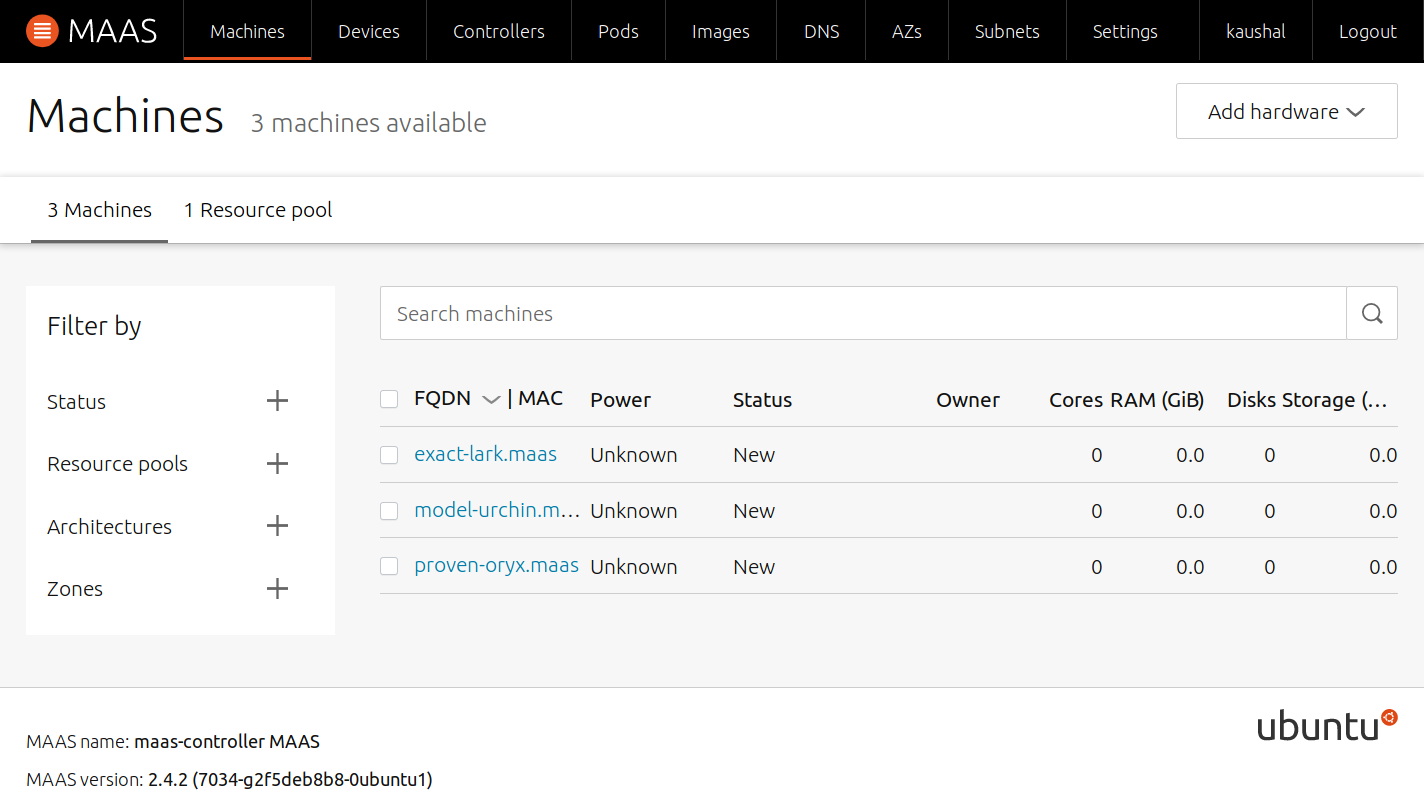
\includegraphics[width=0.7\textwidth]{images/5-4.png}
    \caption{Change these names to the meaningful names}
\end{figure}

\begin{figure}[!ht]
    \centering
    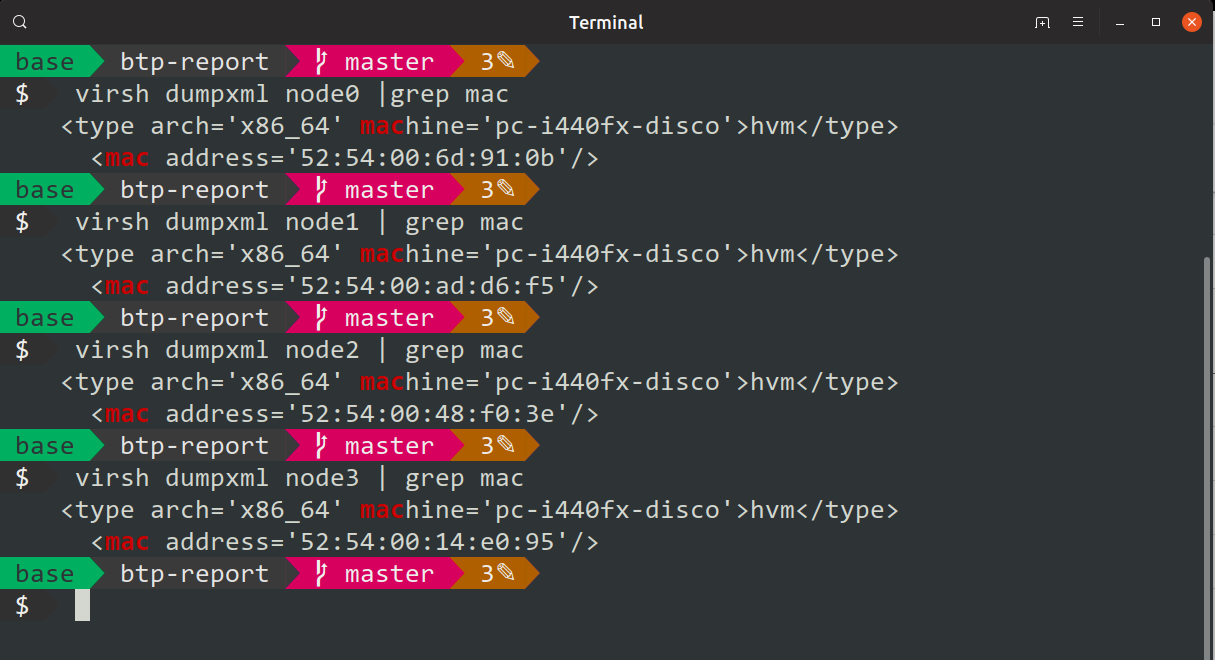
\includegraphics[width=0.7\textwidth]{images/5-5.png}
    \caption{Finding the mac address of each node}
\end{figure}

Once the names are changed, navigate to the power configuration under the configuration tab for each node and set the power parameters as follows:

Power type: Virsh

Virsh Address: \url{qemu+ssh://<USERNAME>@<IP>/system}

Virsh VM ID: \url{node0}

Where USERNAME is related to the host machine and the IP is the local ip of that host machine. For my case USERNAME is `kaushal' and IP is `10.128.1.220'.

\begin{figure}[!ht]
    \centering
    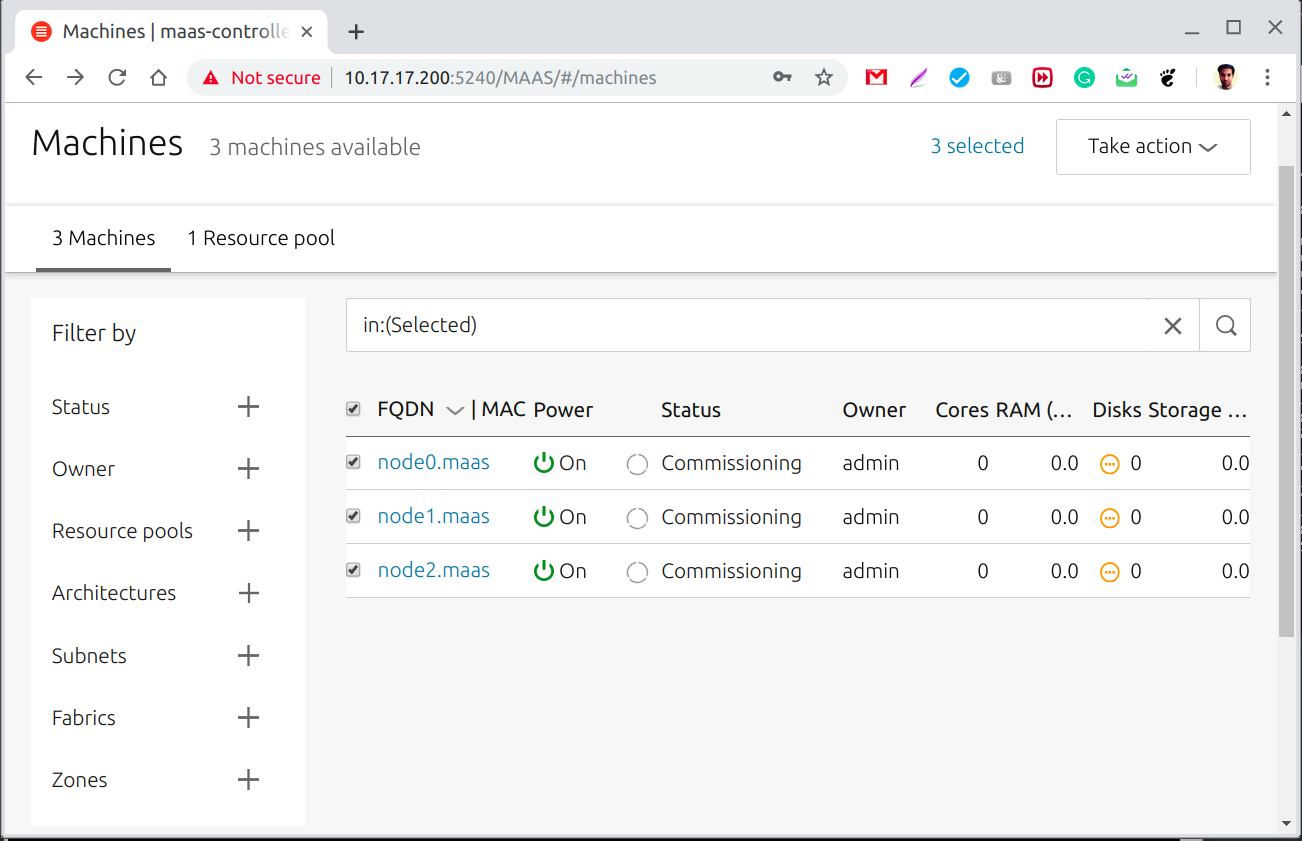
\includegraphics[width=0.7\textwidth]{images/5-6.png}
    \caption{Power configuration for node0}
\end{figure}

\section{Commissioning the nodes}

Once the power configuration is done select all nodes and commission all of them (fig 5.7). During the commissioning procedure the machine will also go through some hardware testing procedure (fig 5.8).

\begin{figure}[!ht]
    \centering
    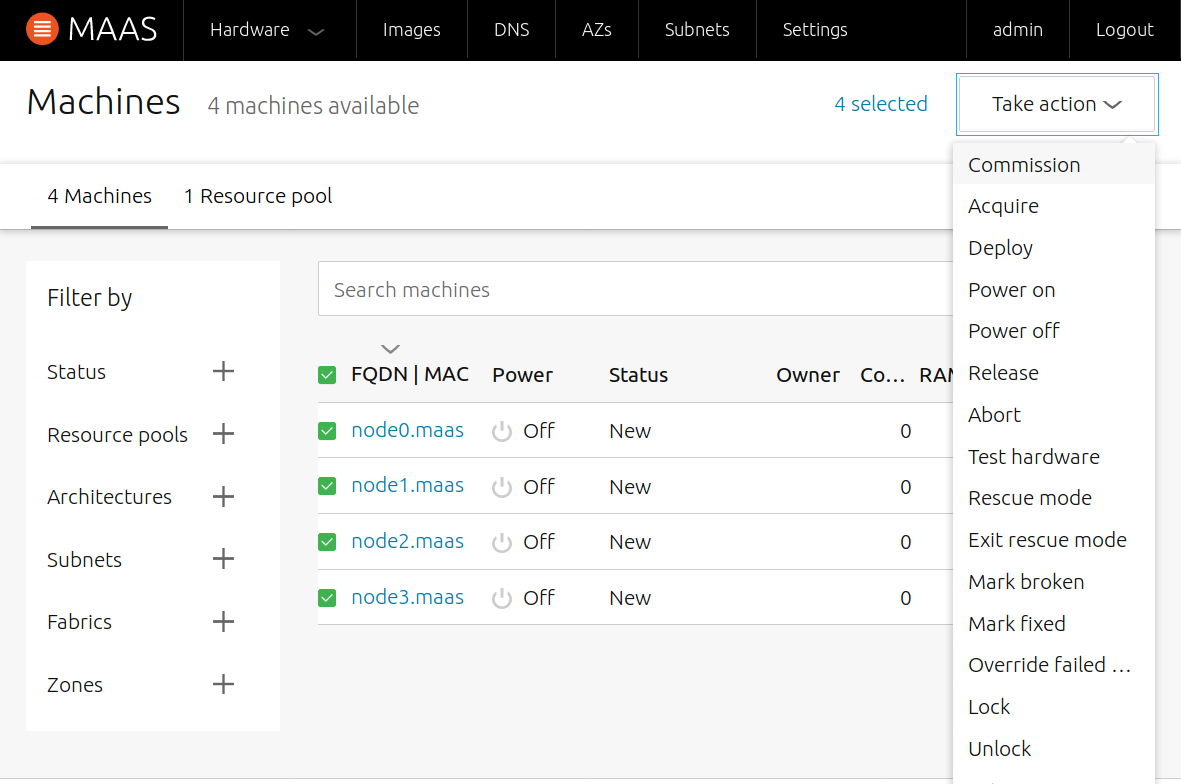
\includegraphics[width=0.7\textwidth]{images/5-7.png}
    \caption{Commissioning all nodes}
\end{figure}

\begin{figure}[!ht]
    \centering
    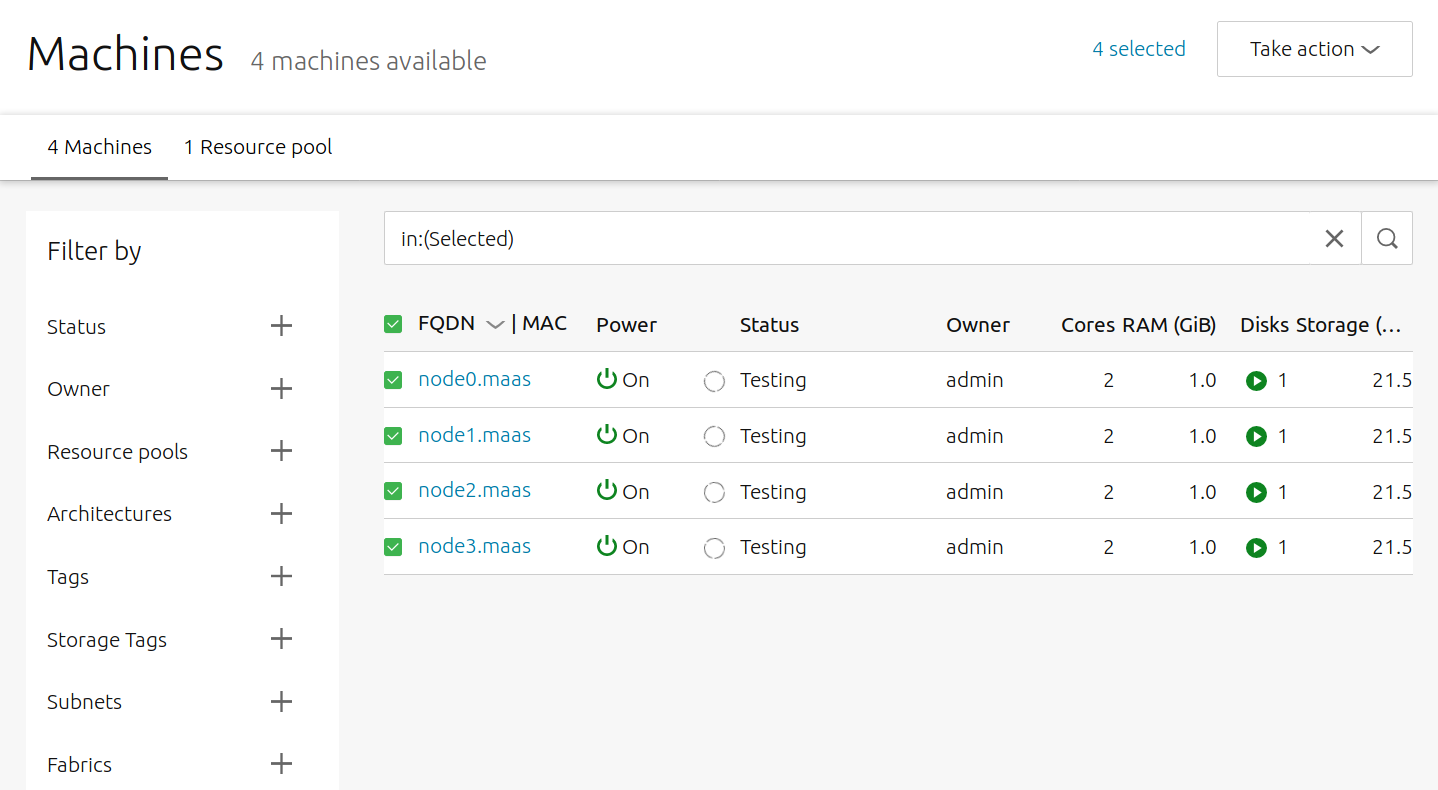
\includegraphics[width=0.7\textwidth]{images/5-8.png}
    \caption{Hardware testing phase}
\end{figure}

Once the commissioning procedure is complete the machines will gracefully shutdown and on the MAAS web interface you will have the basic hardware specification(fig. 5.9).

\begin{figure}[!ht]
    \centering
    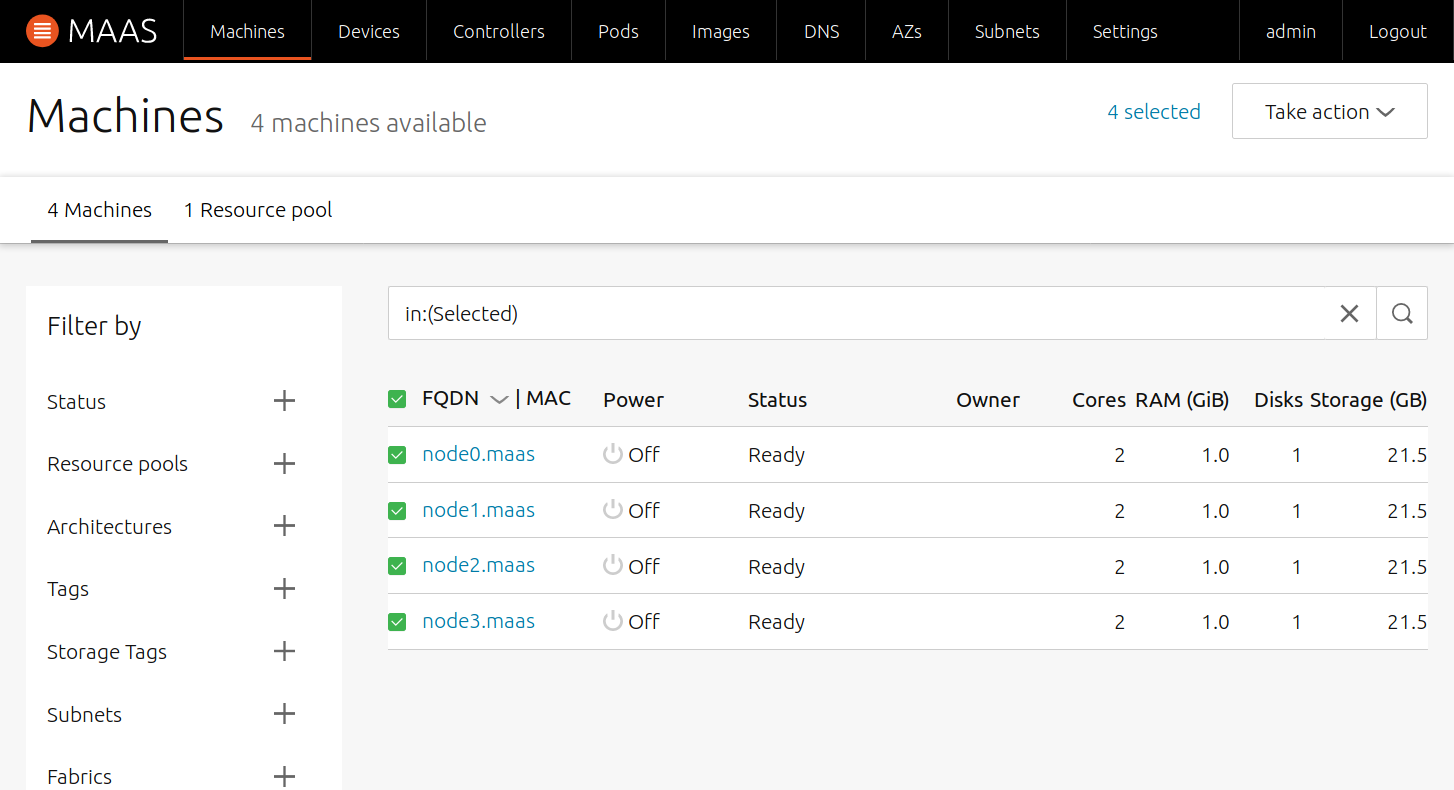
\includegraphics[width=0.7\textwidth]{images/5-9.png}
    \caption{Hardware information}
\end{figure}

This is a basic procedure of how to create MAAS nodes and commission them.

In the next chapter we will discuss the machine acquisition and deployment.